\chapter{EXPERIMENTS AND EVALUATION}
\label{chap:experiment}

\section{Research Questions}

The experiments in this chapter are designed to answer the following research questions:

\begin{itemize}
    \item \textbf{RQ1:} Does the proposed attribute-guided H-CAST improve hierarchical bird classification compared with the image-only H-CAST baseline under the official CUB-200-2011 train/test protocol?

    \item \textbf{RQ2:} Does using a compact selected attribute subset preserve or improve performance compared with using all 312 CUB attributes?

    \item \textbf{RQ3:} Does the proposed HSDAS strategy outperform equally sized random subsets and the internal Sibling-IVAS statistical baseline?

    \item \textbf{RQ4:} How do the proposed attribute-guided components, including species-level fusion, auxiliary attribute prediction, and diversity regularization, affect species accuracy, Full-Path Accuracy, wAP, TICE, and attribute prediction accuracy?
\end{itemize}

These questions correspond directly to the main goals of this thesis. RQ1 evaluates whether attribute-guided learning improves the image-only hierarchical baseline. RQ2 studies whether the proposed hard-sibling-aware attribute selection is more effective than using all attributes, random subsets, or earlier internal selection baselines that do not explicitly model hard siblings. RQ3 analyzes the role of the diversity regularization term. RQ4 examines how the attribute branch contributes to the final prediction behavior, including both classification performance and auxiliary attribute prediction quality.


\section{Dataset and Experimental Protocol}

This section describes the dataset, taxonomy structure, attribute annotations, train/test protocol, and implementation details used in the experiments. The main experiments are conducted on the CUB-200-2011 dataset and follow the official train/test split used in the H-CAST benchmark. This choice ensures that the results are directly comparable with the image-only H-CAST baseline and the reported results of the original H-CAST paper.


\subsection{CUB-200-2011}

The experiments are conducted on the Caltech-UCSD Birds-200-2011 dataset, commonly referred to as CUB-200-2011 \cite{wah2011cub}. CUB-200-2011 is a standard benchmark for fine-grained bird image classification. It contains 200 bird species and 11,788 images. The official split consists of 5,994 training images and 5,794 test images.

CUB-200-2011 is suitable for this thesis for three reasons. First, it is a fine-grained classification dataset where many classes are visually similar and differ only in subtle local traits. Second, the dataset provides rich attribute annotations describing bird appearance, which makes it possible to study attribute-guided representation learning. Third, the bird species can be organized into a biological taxonomy, allowing the task to be formulated as hierarchical classification rather than flat species classification.

In this thesis, each input image is associated with three taxonomic labels: order, family, and species. The model is trained to predict all three levels. The species label is the finest and most difficult prediction target, while family and order represent coarser taxonomic levels.


\subsection{Taxonomy and Attribute Annotations}

Following the H-CAST setting, the CUB-200-2011 species are organized into a three-level hierarchy consisting of 13 orders, 38 families, and 200 species \cite{park2025visually}. Each species belongs to exactly one family, and each family belongs to exactly one order. Therefore, each image has a valid taxonomy path:
\begin{equation}
    y^{o} \rightarrow y^{f} \rightarrow y^{s},
\end{equation}
where \(y^{o}\), \(y^{f}\), and \(y^{s}\) denote the order, family, and species labels, respectively.

In addition to class labels, CUB-200-2011 provides 312 visual attributes. These attributes describe bird traits such as bill shape, wing color, breast pattern, tail shape, head pattern, eye color, belly color, crown color, and other part-based properties. In this thesis, the 312 attributes are organized into 28 semantic groups based on their attribute names. Each group corresponds to one type of bird trait, and each attribute within a group represents one possible state of that trait.

The proposed model does not use attributes as manual inputs during inference. Instead, class-level attribute annotations are used during training as auxiliary supervision. For an image belonging to species \(c\), the attribute target is obtained from the class-level attribute vector of that species. This setting is consistent with the goal of improving image-based hierarchical classification without requiring users to provide attribute labels at test time.

Several attribute usage strategies are evaluated in this chapter. \textbf{FullAttr-312} uses all 312 CUB attributes. \textbf{Sibling-IVAS-188} is an internal node-vs-siblings statistical selection baseline implemented during this thesis. It uses train-only image-level binary attribute annotations and ranks attributes primarily by positive occurrence-rate difference between a target taxonomy node and its corresponding negative set, with Information Value used as a secondary criterion. \textbf{HSDAS-199} selects attributes based on species-level hard-sibling discrimination using class-level continuous attribute profiles. \textbf{Random-199} is used as a control to test whether the benefit comes from the HSDAS selection criterion or merely from reducing the number of attributes.


\subsection{Train/Test Protocol}

The main results in this thesis follow the official CUB-200-2011 train/test protocol. The model is trained on the official training split and evaluated on the official test split. No separate validation set is used for the main reported comparison. This choice follows the experimental setting of H-CAST and allows a direct comparison between the proposed attribute-guided model and the image-only H-CAST baseline.

This protocol is important because the original CUB-200-2011 benchmark and the H-CAST experiments report results using the official train/test split. If a separate validation set were created by splitting the training set, the model would be trained on fewer images, and the resulting numbers would not be directly comparable to the H-CAST baseline trained on the full official training split. Therefore, all main tables in this chapter are reported under the official train/test setting.



\subsection{Implementation Details}

The implementation is based on the original CAST/H-CAST codebase. The H-CAST backbone and the hierarchical visual parsing pipeline are reused and adapted for the CUB-200-2011 setting. The main components implemented in this thesis are the attribute-group representation, HSDAS attribute selection, attribute-group queries, group-specific attribute prediction heads, species-level attribute fusion, and the attribute attention diversity loss.

Unless otherwise specified, the experiments use the \texttt{cast\_small} model configuration. The model uses a convolutional stem, a patch size of 8, an embedding dimension of 384, and four hierarchical stages. The numbers of graph clusters are set to \([64, 32, 16, 8]\), and the Transformer block depths are \([3, 3, 3, 2]\). The model predicts three hierarchy levels: species, family, and order.

For attribute-guided experiments, the attribute mask is loaded before model construction. If a selected attribute mask is provided, only the retained attribute states are used to define the active attribute groups and the output dimensions of the group-specific attribute classifiers. If no mask is provided, the model uses all 312 attributes grouped into the original 28 CUB attribute groups.

The training objective consists of hierarchical classification loss, auxiliary attribute prediction loss, optional Tree-Path KL divergence loss, and optional attribute attention diversity loss. The attribute loss weight is denoted by \(\lambda_{attr}\), and the diversity loss weight is denoted by \(\lambda_{div}\). The default attribute-guided setting uses \(\lambda_{attr}=0.5\). Different values of \(\lambda_{div}\) are evaluated in the ablation study.

The model is trained using the AdamW optimizer with cosine learning-rate scheduling. Standard data augmentation techniques from the H-CAST/DeiT training pipeline are used, including random augmentation, Mixup, CutMix, label smoothing, and random erasing when enabled by the training configuration. The input image size is \(224 \times 224\). Evaluation is performed on the official test set using the image and its corresponding superpixel segmentation input required by the CAST/H-CAST backbone.

During training, the model receives images, superpixel segmentations, taxonomy labels, and class-level attribute targets. During inference, the model receives only the image because the superpixel segmentation required by CAST/H-CAST is generated automatically from the image and no ground-truth attribute labels are provided at inference time.






\section{Compared Methods}

This section describes the methods compared in the experiments. All reported results in the main comparison are obtained under the official CUB-200-2011 train/test protocol.

The compared methods are divided into three groups. The first group contains image-only baselines. The second group contains attribute-guided model variants. The third group compares different attribute selection strategies used to construct the attribute supervision mask.

\subsection{Image-only Baselines}

The image-only baselines do not use CUB attribute annotations during training or inference. They are included to evaluate whether attribute-guided learning provides additional benefit over a standard hierarchical image classifier.

\textbf{H-CAST reported by the authors.} This is the result reported in the original H-CAST paper. It serves as the external reference point for the image-only hierarchical classification setting. Since this result comes from the original paper, it is included only for comparison and is not produced by the implementation in this thesis.

\textbf{H-CAST rerun.} This baseline is obtained by rerunning the image-only H-CAST model under the same CUB train/test protocol used in this thesis. It is the most important image-only baseline because it is trained and evaluated in the same experimental environment as the proposed attribute-guided models. Comparing against this rerun helps separate the effect of the proposed attribute module from differences caused by implementation or training environment.

\begin{table}[t]
    \centering
    \caption{Image-only baselines used for comparison. Results are reported under the official CUB train/test protocol.}
    \label{tab:image_only_baselines}
    \begin{tabular}{l p{8.5cm}}
        \hline
        \textbf{Method} & \textbf{Description} \\
        \hline
        H-CAST reported by authors & Image-only H-CAST result reported in the original paper. Used as an external reference. \\
        H-CAST rerun & Image-only H-CAST model rerun in this thesis under the same CUB train/test protocol. Used as the main image-only baseline. \\
        \hline
    \end{tabular}
\end{table}

\subsection{Attribute-guided Variants}

The attribute-guided variants extend the image-only H-CAST model by adding attribute-oriented learning to the species-level branch. In all these variants, attribute labels are used only during training. During inference, the model receives only the input image and the superpixel segmentation required by the H-CAST/CAST backbone.

\textbf{Attribute-guided H-CAST.} This is the main model proposed in this thesis. It uses one learnable query for each active attribute group. These queries attend to species-level graph-node features and produce attribute-oriented representations. The representations are supervised by group-specific attribute classifiers and are also fused with the species-level class token before species prediction.

\textbf{Attribute-guided H-CAST without diversity loss.} This variant removes the attribute attention diversity loss by setting \(\lambda_{div}=0\). It is used to evaluate whether the diversity regularization term contributes to the final performance.

\textbf{Attribute-guided H-CAST with diversity loss.} This variant enables the diversity term with \(\lambda_{div}>0\). It is used to evaluate whether encouraging different attribute macro-parts to attend to complementary graph nodes improves fine-grained classification.


\begin{table}[t]
    \centering
    \caption{Attribute-guided variants considered in the experiments.}
    \label{tab:attr_guided_variants}
    \small
    \setlength{\tabcolsep}{4pt}
    \renewcommand{\arraystretch}{1.15}
    \begin{tabularx}{\textwidth}{@{}p{3.8cm}ccX@{}}
        \hline
        \textbf{Variant} & \(\lambda_{attr}\) & \(\lambda_{div}\) & \textbf{Purpose} \\
        \hline
        Attribute-guided H-CAST w/o diversity 
        & 0.5 & 0.0 
        & Tests the effect of attribute supervision and species-level fusion without diversity regularization. \\

        Attribute-guided H-CAST with diversity 
        & 0.5 & 0.5 
        & Main proposed setting with attribute supervision, species-level fusion, and diversity loss. \\

        Attribute-guided H-CAST with weak diversity 
        & 0.5 & 0.1 
        & Tests whether a smaller diversity weight gives a better trade-off. \\

        Attribute-guided H-CAST with stronger diversity 
        & 0.5 & 1.0 
        & Tests whether stronger diversity regularization improves or hurts performance. \\
        \hline
    \end{tabularx}
\end{table}

\subsection{Attribute Selection Variants}

This thesis evaluates several ways of choosing the attribute subset used by the attribute-guided module. These variants are important because CUB contains 312 attributes, but not all of them are equally useful for species-level discrimination.

\textbf{FullAttr-312.} This setting uses all 312 CUB attributes. It preserves the full semantic information available in the dataset, but may include redundant or weakly discriminative attributes.

\textbf{HSDAS-199.} This is the main attribute selection strategy studied in this thesis. HSDAS selects attributes at the species level by combining general sibling discriminativeness and hard-sibling discriminativeness. It uses class-level continuous attribute profiles and prioritizes attributes that distinguish a species from sibling species with similar attribute profiles.

\textbf{HSDAS-174.} This variant uses a smaller HSDAS-selected subset. It is included to analyze how attribute subset size affects classification performance.

\textbf{Sibling-IVAS-188.} This is an internal statistical attribute-selection baseline implemented during this thesis. It uses train-only image-level binary attribute annotations and compares each taxonomy node with a corresponding negative set. For species-level nodes, the negative set consists of sibling species within the same family. Attributes are ranked primarily by positive occurrence-rate difference between the target node and the negative set, with Information Value used as a secondary criterion. This baseline is included to compare HSDAS against another taxonomy-aware but non-hard-sibling selection strategy.

\textbf{Random-199.} This setting selects 199 random attributes, matching the number of attributes in HSDAS-199. It is used as a control to test whether performance changes come from the HSDAS selection criterion or merely from reducing the number of attributes.

\begin{table}[t]
    \centering
    \caption{Attribute selection variants compared in this thesis. All variants are evaluated under the official CUB train/test protocol.}
    \label{tab:attr_selection_variants}
    \begin{tabular}{l c p{8cm}}
        \hline
        \textbf{Method} & \textbf{\#Attr} & \textbf{Description} \\
        \hline
        FullAttr-312 & 312 & Uses all CUB attributes. \\
        HSDAS-199 & 199 & Main hard-sibling-aware selected subset using class-level continuous attributes. \\
        HSDAS-174 & 174 & Smaller HSDAS-selected subset for subset-size analysis. \\
        Sibling-IVAS-188 & 188 & Internal train-only node-vs-siblings statistical baseline using positive occurrence-rate difference and Information Value. \\
        Random-199 & 199 & Random subset control with the same size as HSDAS-199. \\
        \hline
    \end{tabular}
\end{table}







\section{Evaluation Metrics}

The models are evaluated using both classification accuracy and hierarchy-consistency metrics, following the H-CAST evaluation protocol \cite{park2025visually}. Since the task is hierarchical, species accuracy alone is not sufficient. A model may predict the correct species, family, or order independently, but the predicted labels may not form a valid taxonomy path. Therefore, this thesis reports level-wise accuracy, Full-Path Accuracy, Weighted Average Precision, Tree-based InConsistency Error, and attribute prediction accuracy.

\subsection{Level-wise Accuracy}

Level-wise accuracy measures the classification accuracy at each taxonomy level independently. In this thesis, the three reported level-wise accuracies are species accuracy, family accuracy, and order accuracy.

Let \(N\) be the number of test samples. For each sample \(i\), let \(y_i^{s}\), \(y_i^{f}\), and \(y_i^{o}\) be the ground-truth species, family, and order labels. Let \(\hat{y}_i^{s}\), \(\hat{y}_i^{f}\), and \(\hat{y}_i^{o}\) be the corresponding predictions. The species accuracy is defined as
\begin{equation}
    Acc_s =
    \frac{1}{N}
    \sum_{i=1}^{N}
    \mathbb{I}
    \left[
        \hat{y}_i^{s} = y_i^{s}
    \right],
\end{equation}
where \(\mathbb{I}[\cdot]\) is the indicator function. Similarly, family accuracy and order accuracy are defined as
\begin{equation}
    Acc_f =
    \frac{1}{N}
    \sum_{i=1}^{N}
    \mathbb{I}
    \left[
        \hat{y}_i^{f} = y_i^{f}
    \right],
\end{equation}
and
\begin{equation}
    Acc_o =
    \frac{1}{N}
    \sum_{i=1}^{N}
    \mathbb{I}
    \left[
        \hat{y}_i^{o} = y_i^{o}
    \right].
\end{equation}

Species accuracy is the main fine-grained classification metric because species is the most specific label. Family and order accuracies measure performance at coarser levels. In the proposed model, the attribute-guided fusion is applied to the species-level branch, so the largest improvement is expected at the species level.

\subsection{Weighted Average Precision}

In addition to level-wise accuracy, this thesis reports weighted Average Precision (wAP), following the H-CAST evaluation protocol. Although named weighted Average Precision following H-CAST, this metric is computed as a class-count-weighted average of level-wise Top-1 accuracies. Let \(L\) be the number of hierarchy levels. For each level \(l\), let \(N_l\) denote the number of classes at that level and let \(P_l\) denote the Top-1 accuracy at that level. The weighted Average Precision is defined as
\begin{equation}
    wAP =
    \sum_{l=1}^{L}
    \frac{N_l}{\sum_{k=1}^{L} N_k}
    P_l.
\end{equation}


This metric weights each level according to the number of classes at that level. For CUB-200-2011, the hierarchy contains 13 orders, 38 families, and 200 species. Therefore, wAP is more strongly influenced by species accuracy than by order or family accuracy. This makes wAP useful as a complementary metric for evaluating hierarchical classification, especially when the finest level contains many more classes than the coarser levels.

However, wAP does not directly measure whether the predicted labels form a valid taxonomy path. Therefore, it should be interpreted together with FPA and TICE. In this thesis, FPA remains the main hierarchical correctness metric, while wAP provides an additional weighted summary of level-wise accuracy.

\subsection{Full-Path Accuracy}

Full-Path Accuracy (FPA) measures whether the model predicts the entire taxonomy path correctly. A prediction is counted as correct only when the species, family, and order labels are all correct.

Formally, FPA is defined as
\begin{equation}
    FPA =
    \frac{1}{N}
    \sum_{i=1}^{N}
    \mathbb{I}
    \left[
        \hat{y}_i^{s}=y_i^{s}
        \land
        \hat{y}_i^{f}=y_i^{f}
        \land
        \hat{y}_i^{o}=y_i^{o}
    \right].
\end{equation}

FPA is stricter than level-wise accuracy because a sample is counted as correct only if all levels are correct simultaneously. This metric is important for hierarchical classification because it evaluates whether the model can produce a fully correct taxonomic prediction. Since family and order accuracies are usually high on CUB, changes in FPA are often strongly influenced by changes in species accuracy.

\subsection{Tree-based InConsistency Error}

Tree-based InConsistency Error (TICE) measures whether the predicted labels form a valid path in the hierarchy. Unlike FPA, TICE does not require the prediction to match the ground truth. Instead, it checks whether the predicted species, family, and order are mutually consistent according to the taxonomy.

Let \(\pi_f(\cdot)\) denote the parent-family mapping from species to family, and let \(\pi_o(\cdot)\) denote the parent-order mapping from family to order. A predicted path is consistent if
\begin{equation}
    \hat{y}_i^{f}
    =
    \pi_f(\hat{y}_i^{s})
    \quad \text{and} \quad
    \hat{y}_i^{o}
    =
    \pi_o(\hat{y}_i^{f}).
\end{equation}

The inconsistency indicator for sample \(i\) is defined as
\begin{equation}
    e_i =
    \mathbb{I}
    \left[
        \hat{y}_i^{f}
        \neq
        \pi_f(\hat{y}_i^{s})
        \;\lor\;
        \hat{y}_i^{o}
        \neq
        \pi_o(\hat{y}_i^{f})
    \right].
\end{equation}

TICE is then computed as
\begin{equation}
    TICE =
    \frac{1}{N}
    \sum_{i=1}^{N}
    e_i.
\end{equation}

A lower TICE indicates better taxonomy consistency. A model can have high level-wise accuracy but still produce inconsistent paths if its species, family, and order heads make predictions that do not correspond to the same taxonomy branch. Therefore, TICE complements accuracy-based metrics by measuring the structural validity of the prediction path.

In the proposed model, TICE is especially useful because the attribute-guided fusion is applied mainly to the species branch. If the species prediction changes without a corresponding change in the family or order predictions, taxonomy inconsistency may increase. Thus, TICE helps analyze the trade-off between improving fine-grained species discrimination and preserving hierarchical consistency.

\subsection{Attribute Prediction Accuracy}

Attribute prediction accuracy evaluates the auxiliary attribute prediction heads. It is reported only for attribute-guided models. Since the model uses group-specific classifiers, attribute accuracy is computed over active attribute groups rather than over a single 312-dimensional binary vector.

For each active group \(g\), the model predicts one retained attribute state. Let \(\hat{t}_{i,g}\) be the predicted attribute state for sample \(i\) and group \(g\), and let \(\tilde{t}_{i,g}\) be the remapped ground-truth attribute target. If the target state is not retained in the selected attribute mask, the sample-group pair is ignored.

For each mini-batch, attribute accuracy is first computed separately for each active group with at least one valid target. Let \(\Omega_g\) denote the set of valid samples for group \(g\) in the mini-batch. The group accuracy is
\begin{equation}
    Acc_{attr}^{g}
    =
    \frac{1}{|\Omega_g|}
    \sum_{i \in \Omega_g}
    \mathbb{I}
    \left[
        \hat{t}_{i,g}
        =
        \tilde{t}_{i,g}
    \right].
\end{equation}

The batch attribute accuracy is then computed as the average over valid groups:
\begin{equation}
    Acc_{attr}^{batch}
    =
    \frac{1}{|\mathcal{G}_{valid}|}
    \sum_{g \in \mathcal{G}_{valid}}
    Acc_{attr}^{g}.
\end{equation}

The reported attribute accuracy is the average of this batch-level attribute accuracy over the test set, weighted by batch size in the evaluation logger.

This metric measures how well the auxiliary attribute heads learn the selected attribute targets. However, attribute prediction accuracy should not be interpreted as the final task performance. A higher attribute accuracy does not always guarantee higher species accuracy, because some attributes may be easy to predict but not highly discriminative for fine-grained species classification. Therefore, attribute accuracy is used as a diagnostic metric to analyze the behavior of the attribute branch, while species accuracy, FPA, wAP, and TICE remain the primary metrics for evaluating hierarchical classification.






\section{Main Results}

This section presents the main comparison between the proposed attribute-guided H-CAST model and image-only baselines under the official CUB-200-2011 train/test protocol. The goal is to answer RQ1: whether attribute-guided learning improves hierarchical bird classification compared with the image-only H-CAST baseline. Unless otherwise stated, the proposed attribute-guided H-CAST refers to the HSDAS-199 setting with \(\lambda_{attr}=0.5\) and \(\lambda_{div}=0.5\).

Table~\ref{tab:main_results} reports Full-Path Accuracy (FPA), level-wise accuracies, Weighted Average Precision (wAP), Tree-based InConsistency Error (TICE), and attribute prediction accuracy when applicable. The image-only baselines do not use attribute annotations and therefore do not report attribute accuracy.

\begin{table}[t]
    \centering
    \caption{Main comparison under the official CUB-200-2011 train/test protocol. Attribute accuracy is reported only for attribute-guided models.}
    \label{tab:main_results}
    \small
    \setlength{\tabcolsep}{4pt}
    \renewcommand{\arraystretch}{1.12}
    \begin{tabularx}{\textwidth}{@{}Xccccccc@{}}
        \hline
        \textbf{Method} & \textbf{FPA} & \textbf{Species} & \textbf{Family} & \textbf{Order} & \textbf{wAP} & \textbf{TICE} & \textbf{Attr} \\
        \hline
        H-CAST authors 
        & 83.28 & 84.86 & 95.12 & 98.65 & 87.13 & 4.12 & -- \\
        H-CAST rerun 
        & 82.86 & 84.55 & 95.22 & 98.74 & 86.90 & 4.35 & -- \\
        \makecell[l]{Proposed attribute-guided\\H-CAST} 
        & \textbf{84.36} & \textbf{85.83} & \textbf{95.62} & \textbf{99.03} & \textbf{88.00} & \textbf{3.62} & 87.04 \\
        \hline
    \end{tabularx}
\end{table}

The proposed attribute-guided H-CAST improves all accuracy-based metrics compared with the H-CAST rerun. Specifically, it improves FPA from 82.86\% to 84.36\%, species accuracy from 84.55\% to 85.83\%, family accuracy from 95.22\% to 95.62\%, order accuracy from 98.74\% to 99.03\%, and wAP from 86.90\% to 88.00\%. It also reduces TICE from 4.35\% to 3.62\%. This result suggests that adding attribute-guided auxiliary supervision and species-level attribute fusion provides useful information beyond the image-only H-CAST baseline.

The largest improvement appears at the species level, which is consistent with the design of the proposed architecture. Attribute-guided fusion is applied to the species-level branch, where fine-grained cues are most important. Since wAP is weighted by the number of classes at each hierarchy level, the improvement in species accuracy also contributes strongly to the improvement in wAP.

Compared with the result reported by the original H-CAST authors, the proposed model also achieves higher FPA, species accuracy, family accuracy, order accuracy, and wAP, while obtaining a lower TICE. However, the comparison with the H-CAST rerun should be considered the primary comparison, because it is produced under the same implementation environment and training setup as the proposed model.

Overall, the main result supports the effectiveness of attribute-guided learning for hierarchical bird classification. Nevertheless, later ablation studies show that the improvement depends on the attribute subset and the loss configuration. Therefore, the proposed method should be interpreted as improving fine-grained species discrimination, while the relationship between species accuracy and taxonomy consistency still requires careful analysis.


\section{Ablation Studies}

This section analyzes the contribution of different components of the proposed method. All ablation studies follow the official CUB-200-2011 train/test protocol. The goal is to understand how attribute selection, attribute subset size, diversity loss, and random attribute selection affect the final performance. 
Unless otherwise stated, attribute-guided variants use species-level fusion with \(\lambda_{attr}=0.5\) and \(\lambda_{div}=0.5\). The diversity-loss ablation varies only \(\lambda_{div}\), while the fusion-design ablation varies the use of fusion, attribute supervision, and diversity regularization.




\subsection{Effect of Attribute Selection}

This ablation evaluates different attribute usage strategies. It addresses RQ2 and RQ3 by comparing compact selected subsets with FullAttr-312 and by comparing HSDAS with Random-199 and Sibling-IVAS-188.

\begin{table}[t]
    \centering
    \caption{Effect of attribute selection strategy under the official CUB train/test protocol. Random-199 is reported as the mean over three random seeds.}
    \label{tab:attr_selection_ablation}
    \scriptsize
    \setlength{\tabcolsep}{3pt}
    \renewcommand{\arraystretch}{1.12}
    \begin{adjustbox}{max width=\textwidth}
    \begin{tabular}{@{}lcccccccc@{}}
        \hline
        \textbf{Method} & \textbf{\#Attr} & \textbf{FPA} & \textbf{Species} & \textbf{Family} & \textbf{Order} & \textbf{wAP} & \textbf{TICE} & \textbf{Attr} \\
        \hline
        FullAttr-312 & 312 & 84.29 & 85.59 & 95.65 & 98.81 & 87.80 & \textbf{3.25} & 85.65 \\
        Sibling-IVAS-188 & 188 & 84.02 & 85.28 & 95.69 & 98.81 & 87.56 & 3.52 & 86.95 \\
        Random-199 mean & 199 & 84.15 & 85.45 & \textbf{95.79} & 98.95 & 87.71 & 3.33 & \textbf{91.28} \\
        HSDAS-199 & 199 & \textbf{84.36} & \textbf{85.83} & 95.62 & \textbf{99.03} & \textbf{88.00} & 3.62 & 87.04 \\
        \hline
    \end{tabular}
    \end{adjustbox}
\end{table}

Among the evaluated attribute usage strategies shown in Table \ref{tab:attr_selection_ablation}, HSDAS-199 achieves the highest species accuracy and wAP. It also achieves higher FPA than FullAttr-312, Sibling-IVAS-188, and the Random-199 mean, although Random-199 seed 2 slightly exceeds it in FPA as discussed later. Compared with FullAttr-312, HSDAS-199 improves species accuracy from 85.59\% to 85.83\% and wAP from 87.80\% to 88.00\%, while using fewer attributes. This suggests that a compact hard-sibling-aware subset can be more useful for species-level discrimination than using all available attributes. However, the improvement over FullAttr-312 is moderate, and FullAttr-312 obtains a lower TICE. Therefore, HSDAS-199 should not be interpreted as strictly better in all aspects.

Compared with Sibling-IVAS-188, HSDAS-199 improves FPA, species accuracy, order accuracy, and wAP. Sibling-IVAS-188 is already a taxonomy-aware internal baseline because it compares each node with sibling-based negative sets. Therefore, the improvement of HSDAS over Sibling-IVAS suggests that explicitly emphasizing hard siblings with similar class-level attribute profiles provides additional benefit for fine-grained species discrimination.

The comparison with Random-199 should be interpreted carefully. HSDAS-199 improves over the Random-199 average in FPA, species accuracy, order accuracy, and wAP. It also achieves higher species accuracy than all three random seeds. However, Random-199 obtains better family accuracy and lower TICE on average, and one random seed obtains slightly higher FPA than HSDAS-199. Therefore, the result supports HSDAS as a useful species-discrimination-oriented selection strategy, but it does not support a strong claim that HSDAS dominates random selection in every metric.

Attribute prediction accuracy is reported only as a diagnostic metric. Random-199 obtains the highest attribute prediction accuracy, but this does not translate into the best species accuracy or wAP. This shows that attribute prediction accuracy and final classification performance are not perfectly correlated. A random subset may contain attribute states that are easier to predict, while HSDAS selects attributes according to hard-sibling discrimination.













\subsection{Effect of Attribute Subset Size}

This ablation studies how the number of selected attributes affects performance. In this experiment, the HSDAS selection strategy is evaluated with different top-\(k\) settings, with the results shown in Table \ref{tab:attr_subset_size}. \textbf{HSDAS-174} is obtained by selecting the top 3 attributes for each species and then taking the union of selected attributes. \textbf{HSDAS-199} is obtained by selecting the top 5 attributes for each species. FullAttr-312 is included as the reference setting that uses all CUB attributes.

\begin{table}[t]
    \centering
    \caption{Effect of HSDAS attribute subset size. HSDAS-174 uses top-3 attributes per species, while HSDAS-199 uses top-5 attributes per species. All settings use the official CUB train/test protocol.}
    \label{tab:attr_subset_size}
    \scriptsize
    \setlength{\tabcolsep}{3pt}
    \renewcommand{\arraystretch}{1.12}
    \begin{adjustbox}{max width=\textwidth}
    \begin{tabular}{@{}lcccccccc@{}}
        \hline
        \textbf{Method} & \textbf{\#Attr} & \textbf{FPA} & \textbf{Species} & \textbf{Family} & \textbf{Order} & \textbf{wAP} & \textbf{TICE} & \textbf{Attr} \\
        \hline
        HSDAS top-3 (174) 
        & 174 & 84.29 & 85.78 & 95.50 & 98.88 & 87.93 & 3.37 & \textbf{87.42} \\
        HSDAS top-5 (199) 
        & 199 & \textbf{84.36} & \textbf{85.83} & 95.62 & \textbf{99.03} & \textbf{88.00} & 3.62 & 87.04 \\
        FullAttr-312 
        & 312 & 84.29 & 85.59 & \textbf{95.65} & 98.81 & 87.80 & \textbf{3.25} & 85.65 \\
        \hline
    \end{tabular}
    \end{adjustbox}
\end{table}

The results show that increasing HSDAS selection from top-3 to top-5 attributes per species gives a small improvement in FPA, species accuracy, order accuracy, and wAP. HSDAS top-5 improves species accuracy from 85.78\% to 85.83\% and wAP from 87.93\% to 88.00\%. The gain is modest, which suggests that HSDAS top-3 already preserves most of the useful attribute supervision.

However, the improvement is not uniform across all metrics. HSDAS top-3 obtains lower TICE and higher attribute prediction accuracy than HSDAS top-5. This suggests that the more compact top-3 subset may be easier for the attribute branch to predict and is associated with lower TICE in this experiment. In contrast, the top-5 subset slightly improves species-level discrimination and wAP but increases TICE.

Compared with FullAttr-312, both HSDAS subsets achieve higher species accuracy and wAP while using fewer attributes. FullAttr-312 provides the best TICE and slightly higher family accuracy, but its species accuracy and wAP are lower than both HSDAS variants.
Overall, HSDAS top-5 is selected as the main proposed setting because it achieves the best species accuracy, FPA, and wAP among the subset-size variants. However, HSDAS top-3 remains a competitive compact alternative, with better attribute prediction accuracy and lower TICE.










\subsection{Effect of Attribute Diversity Loss}

This ablation evaluates the role of the attribute attention diversity loss. It contributes to RQ4 by analyzing how diversity regularization affects species accuracy, FPA, wAP, and taxonomy consistency.

\begin{table}[t]
    \centering
    \caption{Effect of the attribute attention diversity loss using HSDAS-199.}
    \label{tab:diversity_loss_ablation}
    \scriptsize
    \setlength{\tabcolsep}{3pt}
    \renewcommand{\arraystretch}{1.12}
    \begin{adjustbox}{max width=\textwidth}
    \begin{tabular}{@{}lcccccccc@{}}
        \hline
        \textbf{Setting} & \(\lambda_{div}\) & \textbf{FPA} & \textbf{Species} & \textbf{Family} & \textbf{Order} & \textbf{wAP} & \textbf{TICE} & \textbf{Attr} \\
        \hline
        HSDAS-199 without diversity 
        & 0.0 & 84.16 & 85.47 & 95.63 & 98.62 & 87.69 & \textbf{3.14} & 87.01 \\
        HSDAS-199 weak diversity 
        & 0.1 & 84.02 & 85.33 & \textbf{95.79} & 98.91 & 87.62 & 3.44 & \textbf{87.46} \\
        HSDAS-199 main setting 
        & 0.5 & \textbf{84.36} & \textbf{85.83} & 95.62 & \textbf{99.03} & \textbf{88.00} & 3.62 & 87.04 \\
        HSDAS-199 strong diversity 
        & 1.0 & 84.04 & 85.33 & 95.75 & 98.79 & 87.60 & 3.40 & 86.12 \\
        \hline
    \end{tabular}
    \end{adjustbox}
\end{table}

The results in Table~\ref{tab:diversity_loss_ablation} suggest that the diversity loss has a non-monotonic effect. The main setting with \(\lambda_{div}=0.5\) achieves the best FPA and species accuracy, suggesting that a moderate amount of diversity regularization can help fine-grained species discrimination. However, weaker diversity \((\lambda_{div}=0.1)\) and stronger diversity \((\lambda_{div}=1.0)\) do not improve species accuracy over the no-diversity setting. Therefore, the results do not support the claim that simply increasing diversity regularization always improves performance.

The no-diversity setting obtains the lowest TICE. This indicates that the model can produce more taxonomically consistent paths when the diversity regularizer is removed. In contrast, the best species accuracy is obtained with \(\lambda_{div}=0.5\), which has higher TICE. This suggests a trade-off between species-level discrimination and taxonomy consistency.

One possible explanation is that the diversity loss is intended to encourage attribute macro-parts to use more complementary graph-node evidence, which may improve species prediction. However, because family and order predictions are not directly fused with attribute features, changes in species prediction may not always be matched by corresponding changes in the coarser predictions. This can increase path inconsistency even when species accuracy improves.

The result with \(\lambda_{div}=1.0\) suggests that too much diversity regularization may become harmful. A strong diversity constraint may force attention maps to spread or separate even when the image contains only a few truly discriminative cues. Therefore, the diversity loss should be treated as a regularizer that requires careful weighting rather than a universally beneficial component.







\subsection{Effect of Attribute Fusion Design}

This ablation directly addresses RQ4 by analyzing the contribution of auxiliary attribute supervision, species-level attribute fusion, and diversity regularization. The results are shown in Table \ref{tab:fusion_design_ablation}.

\begin{table}[t]
    \centering
    \caption{Effect of attribute supervision, species-level fusion, and diversity regularization under the official CUB train/test protocol.}
    \label{tab:fusion_design_ablation}
    \scriptsize
    \setlength{\tabcolsep}{3pt}
    \renewcommand{\arraystretch}{1.12}
    \begin{adjustbox}{max width=\textwidth}
    \begin{tabular}{@{}lccccccc@{}}
        \hline
        \textbf{Method} & \textbf{FPA} & \textbf{Species} & \textbf{Family} & \textbf{Order} & \textbf{wAP} & \textbf{TICE} & \textbf{Attr} \\
        \hline
        H-CAST rerun 
        & 82.86 & 84.55 & 95.22 & 98.74 & 86.90 & 4.35 & -- \\

        \makecell[l]{No fusion\\ \(\lambda_{attr}=0.5,\lambda_{div}=0\)}
        & 83.09 & 84.38 & 95.58 & 98.72 & 86.82 & 3.54 & \textbf{89.04} \\

        \makecell[l]{Fusion\\ \(\lambda_{attr}=0,\lambda_{div}=0\)}
        & 83.73 & 85.21 & 95.53 & 98.74 & 87.47 & 3.87 & 23.02 \\

        \makecell[l]{Fusion\\ \(\lambda_{attr}=0.5,\lambda_{div}=0\)}
        & 84.16 & 85.47 & \textbf{95.63} & 98.62 & 87.69 & \textbf{3.14} & 87.01 \\

        \makecell[l]{Fusion\\ \(\lambda_{attr}=0.5,\lambda_{div}=0.5\)}
        & \textbf{84.36} & \textbf{85.83} & 95.62 & \textbf{99.03} & \textbf{88.00} & 3.62 & 87.04 \\
        \hline
    \end{tabular}
    \end{adjustbox}
\end{table}

The no-fusion setting shows that auxiliary attribute supervision alone is not sufficient to improve species classification. Although this setting obtains the highest attribute prediction accuracy, its species accuracy is 84.38\%, which is slightly lower than the H-CAST rerun. This indicates that learning to predict attributes does not automatically transfer to better species recognition unless attribute-oriented features are explicitly connected to the species classifier.

The comparison between the no-fusion setting and the fusion setting with \(\lambda_{attr}=0.5\), \(\lambda_{div}=0\) shows the importance of species-level fusion. With the same attribute supervision weight and no diversity loss, adding fusion improves FPA from 83.09\% to 84.16\%, species accuracy from 84.38\% to 85.47\%, and wAP from 86.82\% to 87.69\%. This supports the design choice of concatenating the attention-pooled attribute summary with the species class token.

The fusion-only setting, where \(\lambda_{attr}=0\), improves species accuracy compared with the no-fusion setting, but its attribute accuracy drops sharply to 23.02\%. This suggests that the additional fusion path can learn classification-useful features through the species classification loss, but these features are not semantically aligned with CUB attributes when attribute supervision is removed.

When attribute supervision is added to the fusion model with \(\lambda_{attr}=0.5\), FPA increases from 83.73\% to 84.16\%, species accuracy increases from 85.21\% to 85.47\%, TICE decreases from 3.87\% to 3.14\%, and attribute accuracy increases from 23.02\% to 87.01\%. This suggests that attribute supervision helps align the fused representation with semantic bird traits and improves taxonomy consistency in the no-diversity setting.

Adding diversity regularization with \(\lambda_{div}=0.5\) further improves FPA, species accuracy, order accuracy, and wAP. The full model achieves the best species accuracy and wAP among the fusion-design settings. However, TICE increases compared with the no-diversity fusion setting, which again indicates a trade-off between fine-grained species discrimination and taxonomy consistency.

Overall, this ablation shows that the proposed model benefits from the combination of attribute supervision and species-level fusion. Attribute supervision alone learns meaningful attribute predictors but does not improve species recognition without fusion. Fusion allows attribute-oriented features to affect the species classifier, while attribute supervision encourages these features to align with the selected CUB attribute targets. The best species accuracy and wAP are obtained when attribute supervision, fusion, and diversity regularization are used together.









\subsection{Random Attribute Control}

Random-199 is used to test whether the performance of HSDAS-199 comes from the hard-sibling-aware selection criterion or simply from using fewer attributes than FullAttr-312. In this thesis, Random-199 is constructed as a group-matched random control. It does not sample 199 attributes uniformly from the full 312-dimensional attribute space. Instead, for each semantic attribute group, it randomly samples the same number of attribute states as the HSDAS-199 mask. Therefore, Random-199 preserves the same group-level structure and active-group coverage as HSDAS-199, while removing the hard-sibling-aware selection criterion.

\begin{table}[t]
    \centering
    \caption{Random attribute control. Random-199 uses the same number of attributes as HSDAS-199 and preserves the same number of selected attribute states per group. Mean and standard deviation are computed over three random seeds.}
    \label{tab:random_control}
    \scriptsize
    \setlength{\tabcolsep}{3pt}
    \renewcommand{\arraystretch}{1.12}
    \begin{adjustbox}{max width=\textwidth}
    \begin{tabular}{@{}lcccccccc@{}}
        \hline
        \textbf{Method} & \textbf{\#Attr} & \textbf{FPA} & \textbf{Species} & \textbf{Family} & \textbf{Order} & \textbf{wAP} & \textbf{TICE} & \textbf{Attr} \\
        \hline
        Random-199 seed 1 
        & 199 & 83.85 & 85.21 & 95.75 & 98.96 & 87.52 & 3.47 & 91.02 \\
        Random-199 seed 2 
        & 199 & 84.40 & 85.66 & 95.86 & 98.95 & 87.89 & 3.42 & 91.06 \\
        Random-199 seed 3 
        & 199 & 84.19 & 85.47 & 95.75 & 98.95 & 87.72 & 3.11 & 91.77 \\
        \makecell[l]{Random-199\\ mean \(\pm\) std}
        & 199 
        & \makecell{84.15\\\(\pm 0.28\)}
        & \makecell{85.45\\\(\pm 0.23\)}
        & \makecell{95.79\\\(\pm 0.06\)}
        & \makecell{98.95\\\(\pm 0.01\)}
        & \makecell{87.71\\\(\pm 0.19\)}
        & \makecell{3.33\\\(\pm 0.20\)}
        & \makecell{91.28\\\(\pm 0.42\)} \\
        HSDAS-199 
        & 199 & \textbf{84.36} & \textbf{85.83} & 95.62 & \textbf{99.03} & \textbf{88.00} & 3.62 & 87.04 \\
        \hline
    \end{tabular}
    \end{adjustbox}
\end{table}

The Random-199 control in Table~\ref{tab:random_control} shows that group-matched random subsets can be competitive. This is expected because Random-199 keeps the same number of attribute states in each semantic group as HSDAS-199. As a result, it still preserves broad coverage over color, shape, pattern, and part-related attribute groups. Therefore, this control is stronger than a purely uniform random subset over all 312 attributes, where the group distribution could become unbalanced.

Random-199 seed 2 obtains slightly higher FPA than HSDAS-199. However, this does not contradict the main conclusion of this thesis. FPA depends on the joint correctness of species, family, and order predictions. HSDAS-199 achieves higher species accuracy than seed 2, improving from 85.66\% to 85.83\%, and also achieves higher wAP, improving from 87.89\% to 88.00\%. These metrics are more directly related to fine-grained species discrimination, which is the main goal of the proposed attribute selection strategy. In contrast, seed 2 obtains higher family accuracy and lower TICE, which can lead to slightly better full-path correctness in this particular run. The FPA difference is only 0.04 percentage points, corresponding to roughly two test images. Therefore, this result is better interpreted as random variation among strong group-matched attribute subsets rather than evidence that random selection is superior.

Across the three random seeds, HSDAS-199 achieves higher species accuracy and wAP than every Random-199 run. It also achieves higher FPA than the Random-199 mean. This suggests that hard-sibling-aware selection provides a useful bias toward attributes that are helpful for species-level recognition. At the same time, the advantage is moderate rather than large. Since Random-199 keeps 199 out of 312 attributes and preserves the same group-level coverage as HSDAS-199, it can still contain many useful attribute states.

The TICE results also show that HSDAS-199 should not be claimed to dominate random selection in every metric. All three Random-199 seeds obtain lower TICE than HSDAS-199. This means that the random subsets can produce more taxonomically consistent prediction paths in some runs, even though they do not achieve the best species accuracy or wAP. This observation is consistent with the broader trend in the ablation studies: improving species-level discrimination does not always lead to the lowest taxonomy inconsistency.

The attribute accuracy of Random-199 is also higher than that of HSDAS-199. This result should be interpreted carefully. Attribute prediction accuracy measures how well the auxiliary heads predict the selected attribute states, but it does not directly measure whether those attributes are useful for species classification. Random masks may include more frequent or easier-to-predict attribute states, allowing the auxiliary attribute heads to achieve higher accuracy. In contrast, HSDAS selects attributes according to hard-sibling discriminativeness, which may produce harder attribute targets but more species-relevant supervision. This explains why HSDAS-199 has lower attribute prediction accuracy than Random-199 but higher species accuracy and wAP.

Overall, the random control shows that attribute subset size and group-level coverage already provide a strong baseline. HSDAS-199 should therefore not be interpreted as outperforming random selection in every metric. Its advantage is more specific: it provides a targeted and interpretable hard-sibling-aware selection strategy that achieves higher species accuracy and wAP than all three group-matched random subsets, while also achieving higher FPA than the Random-199 mean.

\section{Qualitative and Diagnostic Analysis}

\subsection{Prediction-Level Case Analysis}

To further analyze the species-level improvement, we compare the prediction outputs of the image-only H-CAST rerun and the proposed attribute-guided model on the CUB test set.

Table~\ref{tab:case_analysis_counts} summarizes the prediction-level case analysis. The proposed model corrects 236 species-level errors made by the H-CAST rerun. Among these corrected cases, 194 correspond to intra-family confusions, where H-CAST predicts the correct family but the wrong species. This accounts for approximately 82.2\% of the corrected species cases. This observation supports the motivation of the proposed hard-sibling-aware attribute selection strategy, because many corrected errors occur between visually related species within the same family.

However, the improvement is not one-sided. The proposed model also introduces 161 new species-level errors where H-CAST was originally correct. This means that the attribute-guided branch changes the species-level decision boundary rather than simply adding correct predictions on top of the baseline. Nevertheless, the number of corrected errors is larger than the number of newly introduced errors, resulting in a net gain of 75 correctly classified species. Over 5,794 test images, this corresponds to approximately 1.29 percentage points, which is consistent with the observed species accuracy improvement from 84.55\% to 85.83\%.

At the same time, there remain 659 images where both models predict the wrong species. This indicates that the proposed attribute-guided module does not eliminate all fine-grained recognition errors. In addition, 86 images are cases where the proposed model predicts the correct species but the full hierarchical path is still inconsistent. This helps explain why the proposed model improves species accuracy and wAP, while its TICE is not the lowest among all ablation settings.

\begin{table}[t]
    \centering
    \caption{Prediction-level case analysis comparing the H-CAST rerun and the proposed attribute-guided model on the CUB test set.}
    \label{tab:case_analysis_counts}
    \footnotesize
    \setlength{\tabcolsep}{3pt}
    \renewcommand{\arraystretch}{1.05}
    \begin{tabularx}{0.92\textwidth}{@{}p{4.0cm} c X@{}}
        \hline
        \textbf{Case type} & \textbf{Count} & \textbf{Interpretation} \\
        \hline
        H-CAST wrong, proposed correct 
        & 236 
        & Species-level errors corrected by the proposed model. \\

        H-CAST wrong within same family, proposed correct 
        & 194 
        & Corrected intra-family species confusions. \\

        H-CAST correct, proposed wrong 
        & 161 
        & Correct baseline predictions lost by the proposed model. \\

        Both models wrong at species level 
        & 659 
        & Remaining hard failure cases. \\

        Proposed species correct but path inconsistent 
        & 86 
        & Species prediction is correct, but the predicted hierarchical path is not fully consistent. \\

        Net species-level gain 
        & +75 
        & Corrected errors minus newly introduced errors. \\
        \hline
    \end{tabularx}
\end{table}

\begin{figure}[t]
    \centering
    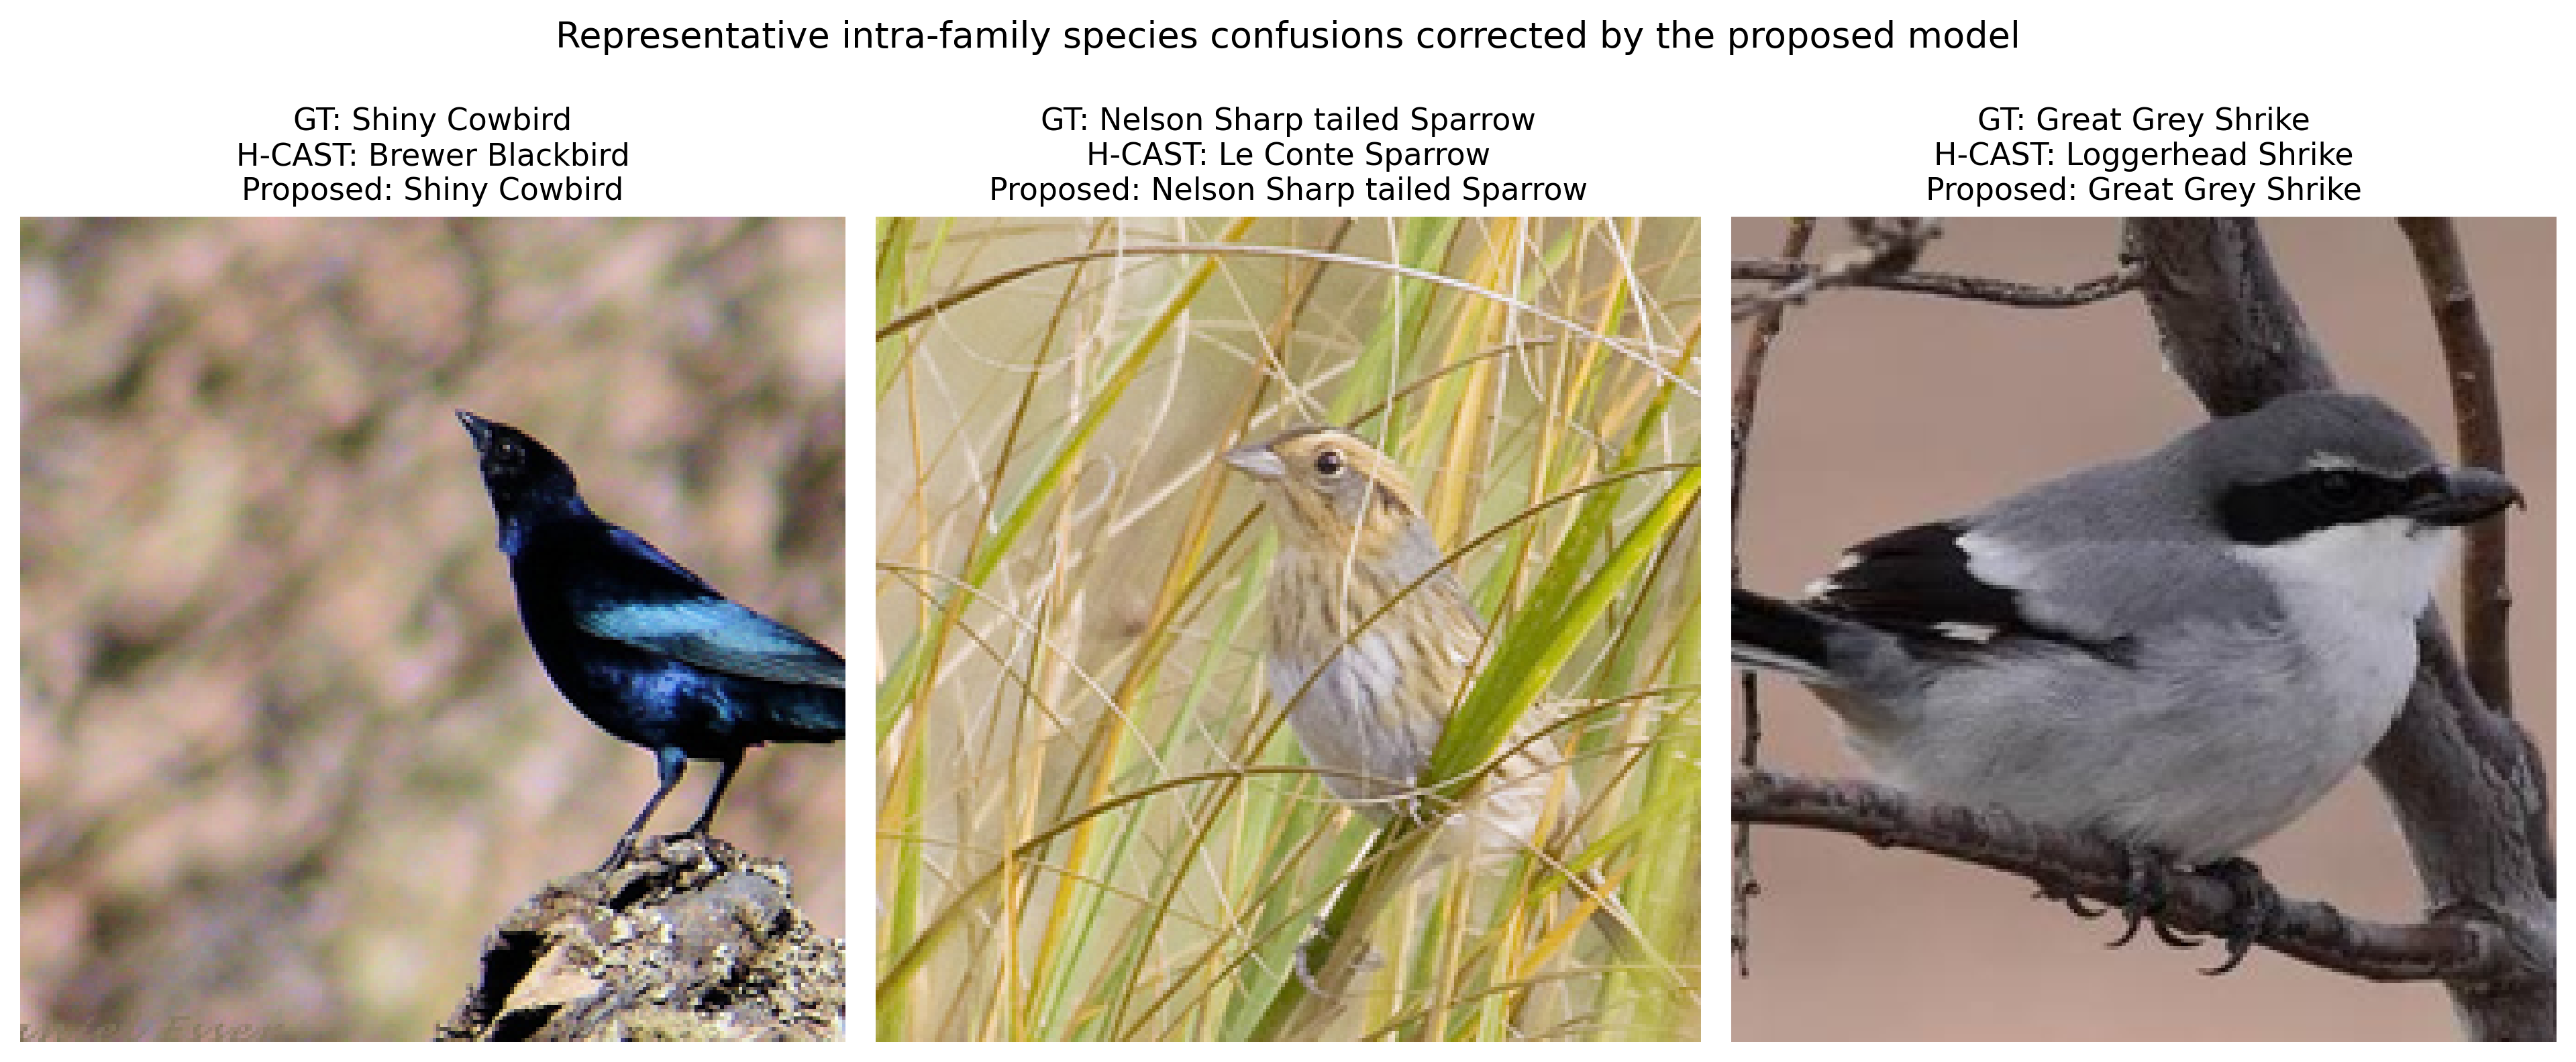
\includegraphics[width=\textwidth]{figures/case_B_examples_model_crop.png}
    \caption{Representative intra-family species confusions corrected by the proposed model. In each example, H-CAST predicts an incorrect species while still predicting the correct family, whereas the proposed attribute-guided model predicts the correct species.}
    \label{fig:case_b_examples}
\end{figure}

Figure~\ref{fig:case_b_examples} shows representative intra-family confusion cases corrected by the proposed model. These examples illustrate the type of errors captured by the second row of Table~\ref{tab:case_analysis_counts}: the image-only H-CAST baseline already predicts the correct family but fails to distinguish the correct species, while the proposed model makes the correct species-level prediction. This supports the quantitative observation that the proposed attribute-guided model is particularly useful for some fine-grained species confusions within the same family.

It should be noted that these examples are illustrative rather than exhaustive. The main evidence for the improvement comes from the prediction-level counts and the quantitative metrics reported in the previous sections.


\subsection{Diagnostic Analysis of Attribute Attention}

In addition to the prediction-level case analysis, we inspect the internal attention behavior of the proposed attribute-guided module. This analysis is intended to provide diagnostic insight into how the attribute branch behaves, rather than to prove that the model accurately localizes semantic attributes.

The proposed module produces two attention signals. First, during species-level fusion, the species class token attends to the attribute-group features through an attention-pooling operation. This produces a distribution over active attribute groups and indicates which groups contribute more strongly to the fused species representation. Second, each attribute-group query cross-attends to the species-level graph nodes generated by the H-CAST backbone. These graph-node attention weights are back-projected to the initial superpixels using the H-CAST graph assignment structure and are overlaid on the input image for visualization.

For the three-level CUB hierarchy used in this thesis, the attribute-group queries attend to the species-level graph representation. The visualized images correspond to the evaluation input after resizing and center cropping, which is the same input view used by the model during inference.

The attention ranking analysis shows that the species-token pooling attention is often dominated by global morphology groups, especially \textit{size} and \textit{shape}. In many inspected examples, these two groups receive substantially higher pooling weights than most other groups. This suggests that the fusion module assigns high importance to global morphology-oriented attribute features. However, these weights should not be interpreted as evidence that the model precisely localizes size or shape in the image. Instead, they indicate that the fused species representation may rely on global cues such as morphology, silhouette, scale, or contextual information.

This behavior is partly related to the selected HSDAS-199 mask. In this mask, the \textit{size} group contains only one retained attribute state, while the \textit{shape} group contains only two retained states. Therefore, these groups provide limited within-group attribute classification supervision, especially for the singleton \textit{size} group. Their queries can still receive gradients through the species-level fusion path, so high CLS pooling weights may reflect classification-useful latent features rather than precisely localized semantic attribute evidence.

Figure~\ref{fig:attention_diagnostic} shows a representative diagnostic visualization. The CLS pooling chart shows the species-token attention over attribute groups. In this example, the highest-weighted groups are \textit{size}, \textit{shape}, and \textit{back pattern}. Since the top-ranked groups are often dominated by global morphology groups, the spatial heatmaps in Figure~\ref{fig:attention_diagnostic}(b) are selected from local or part-related groups for diagnostic inspection. These maps allow us to examine whether some attribute queries attend to plausible bird regions. In some examples, local attribute-query maps overlap with the bird body or discriminative parts. However, this behavior is not sufficiently consistent to support a strong claim of semantic attribute localization.

\begin{figure}[t]
    \centering

    \begin{subfigure}{0.95\textwidth}
        \centering
        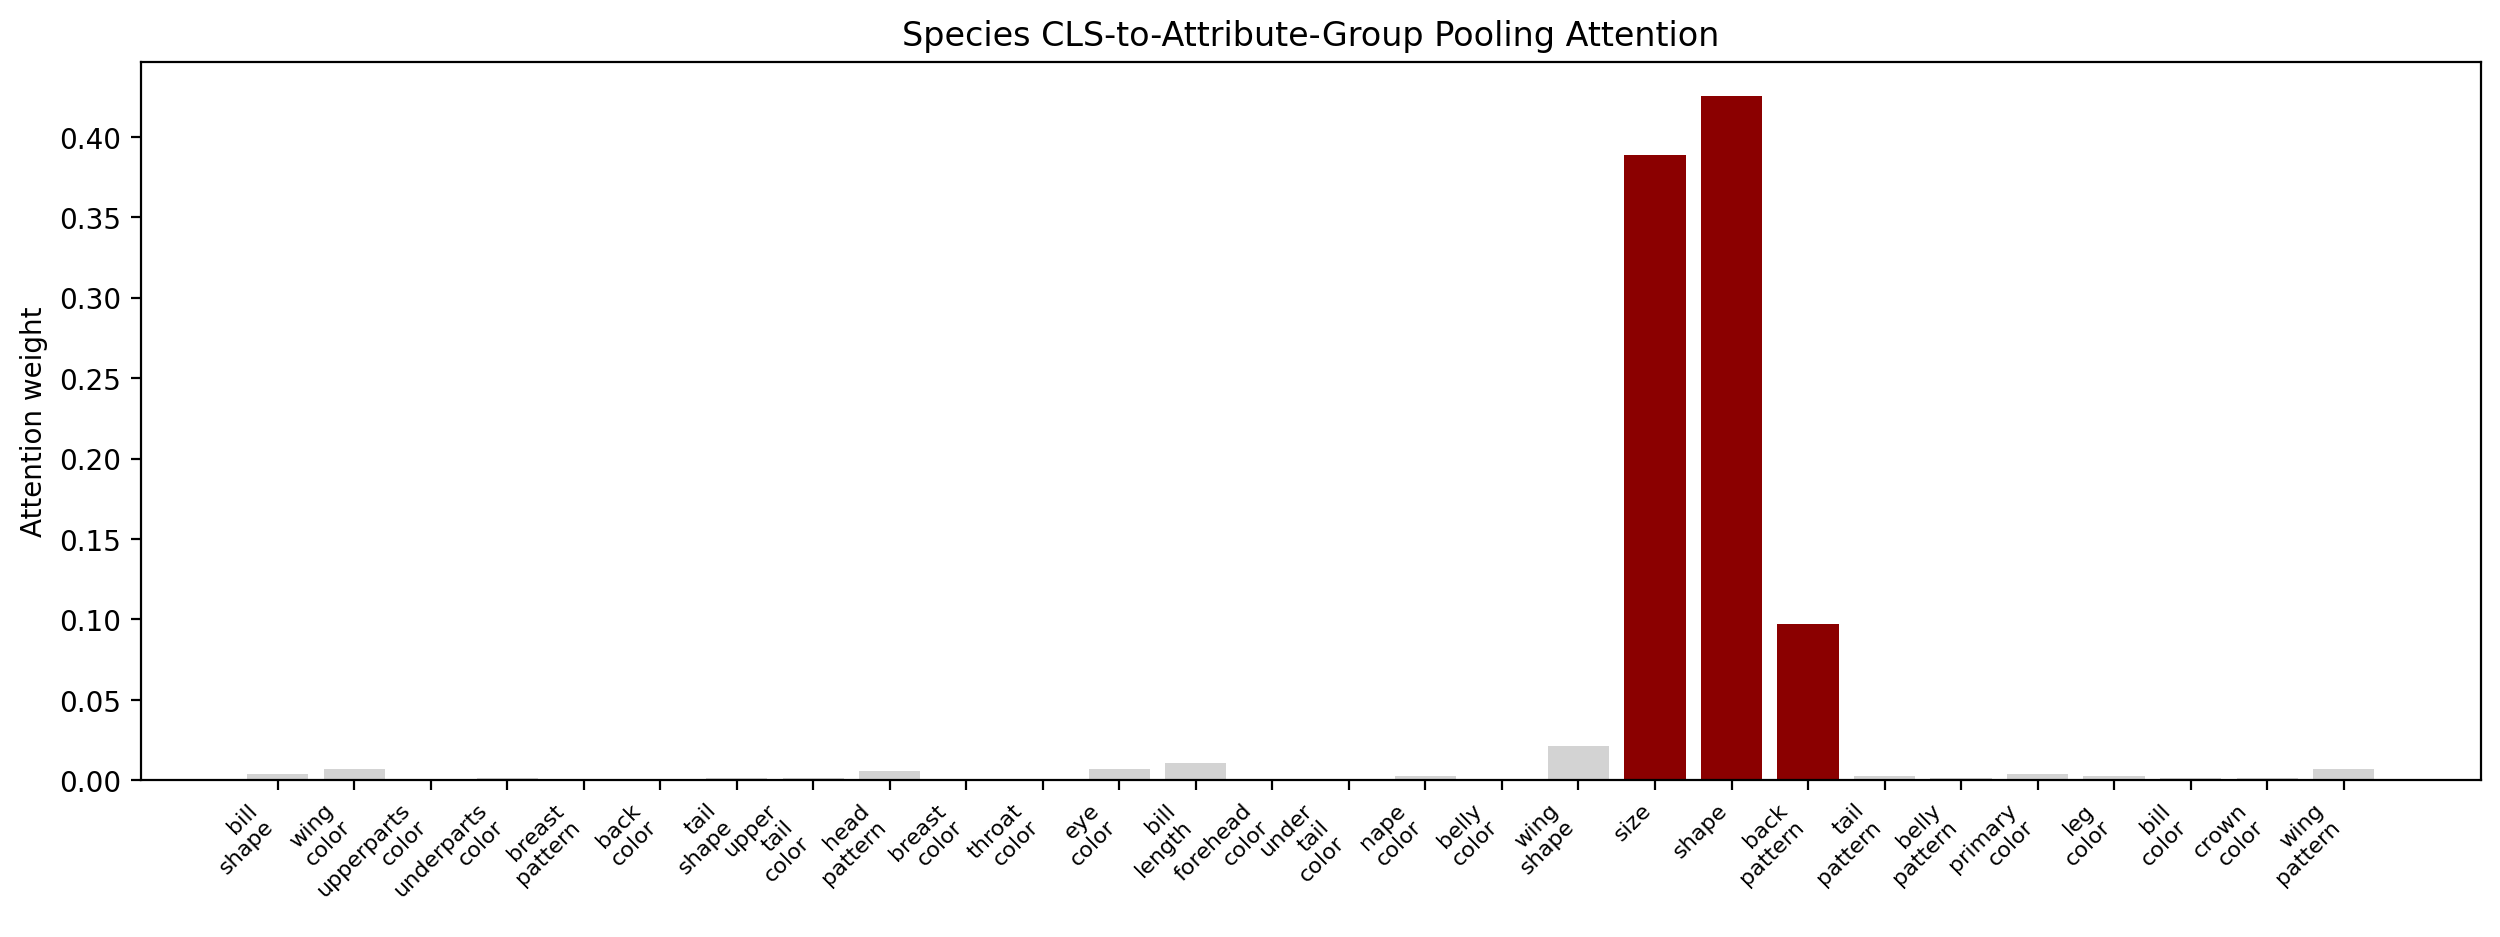
\includegraphics[width=\textwidth]{figures/case_California_Gull_0038_40865_cls_pooling.png}
        \caption{Species CLS-to-attribute-group pooling attention.}
        \label{fig:attention_diagnostic_cls}
    \end{subfigure}

    \vspace{0.5em}

    \begin{subfigure}{0.95\textwidth}
        \centering
        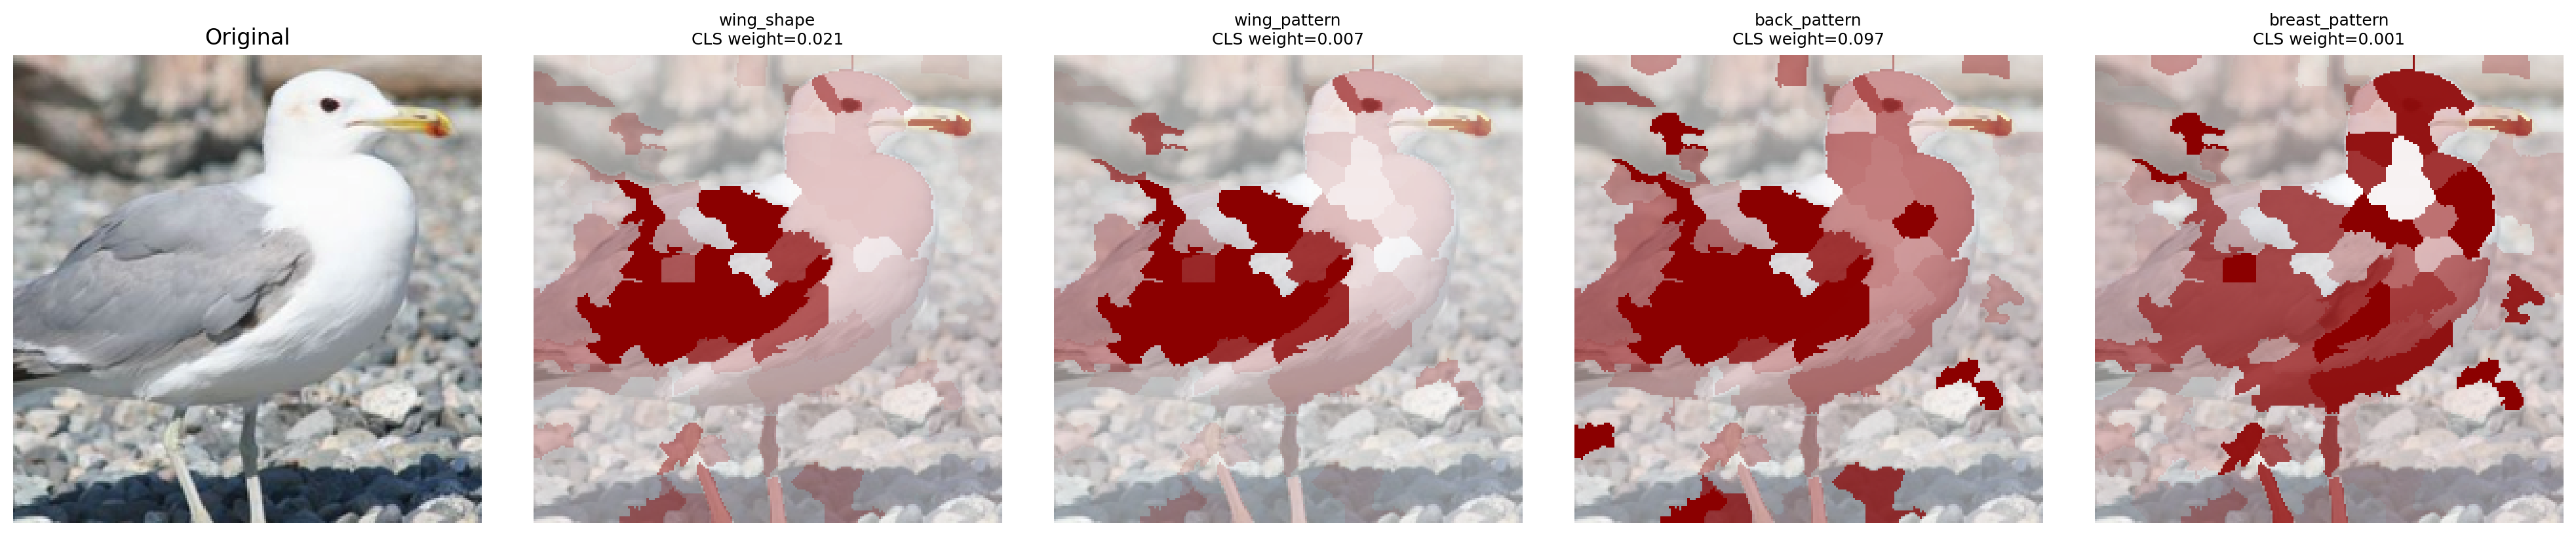
\includegraphics[width=\textwidth]{figures/case_California_Gull_0038_40865_attr_graph_top3_hard.png}
        \caption{Selected attribute-query spatial attention maps.}
        \label{fig:attention_diagnostic_spatial}
    \end{subfigure}

    \caption[Diagnostic visualization of the attribute-guided module.]
    {Diagnostic visualization of the attribute-guided module. 
    (a) The CLS pooling chart shows the species-token attention over attribute groups. In this example, the three highest-weighted groups are \textit{size}, \textit{shape}, and \textit{back pattern}, indicating that the fusion module assigns strong weight to global morphology-related groups. 
    (b) The spatial heatmaps show selected attribute-query attention maps back-projected to image superpixels. From left to right, the maps correspond to the original image, \textit{wing shape}, \textit{wing pattern}, \textit{back pattern}, and \textit{breast pattern}. These local or part-related groups are selected for diagnostic inspection and are not necessarily the highest-ranked groups in the CLS pooling distribution. These visualizations should not be interpreted as ground-truth attribute localization.}
    \label{fig:attention_diagnostic}
\end{figure}

The spatial attention maps of high-weight global groups further reveal a limitation of the current method. Although \textit{size} and \textit{shape} often receive high pooling weights, their graph-node attention maps are not consistently aligned with a clearly localized semantic part. In some inspected examples, these maps overlap with the bird body or head region, while in other cases they become diffuse or include substantial background regions. Therefore, high pooling weight for global morphology groups should not be interpreted as reliable evidence of precise attribute localization.

Figure~\ref{fig:size_shape_background_example} shows one representative limitation case. In this example, the \textit{size} and \textit{shape} attention maps place a substantial portion of their response on background regions instead of being tightly concentrated on the bird itself. This illustrates that even when these groups receive high CLS pooling weights, the corresponding spatial maps may still reflect a mixture of object cues, silhouette, scale, and contextual information rather than a precisely localized semantic attribute.

\begin{figure}[t]
    \centering
    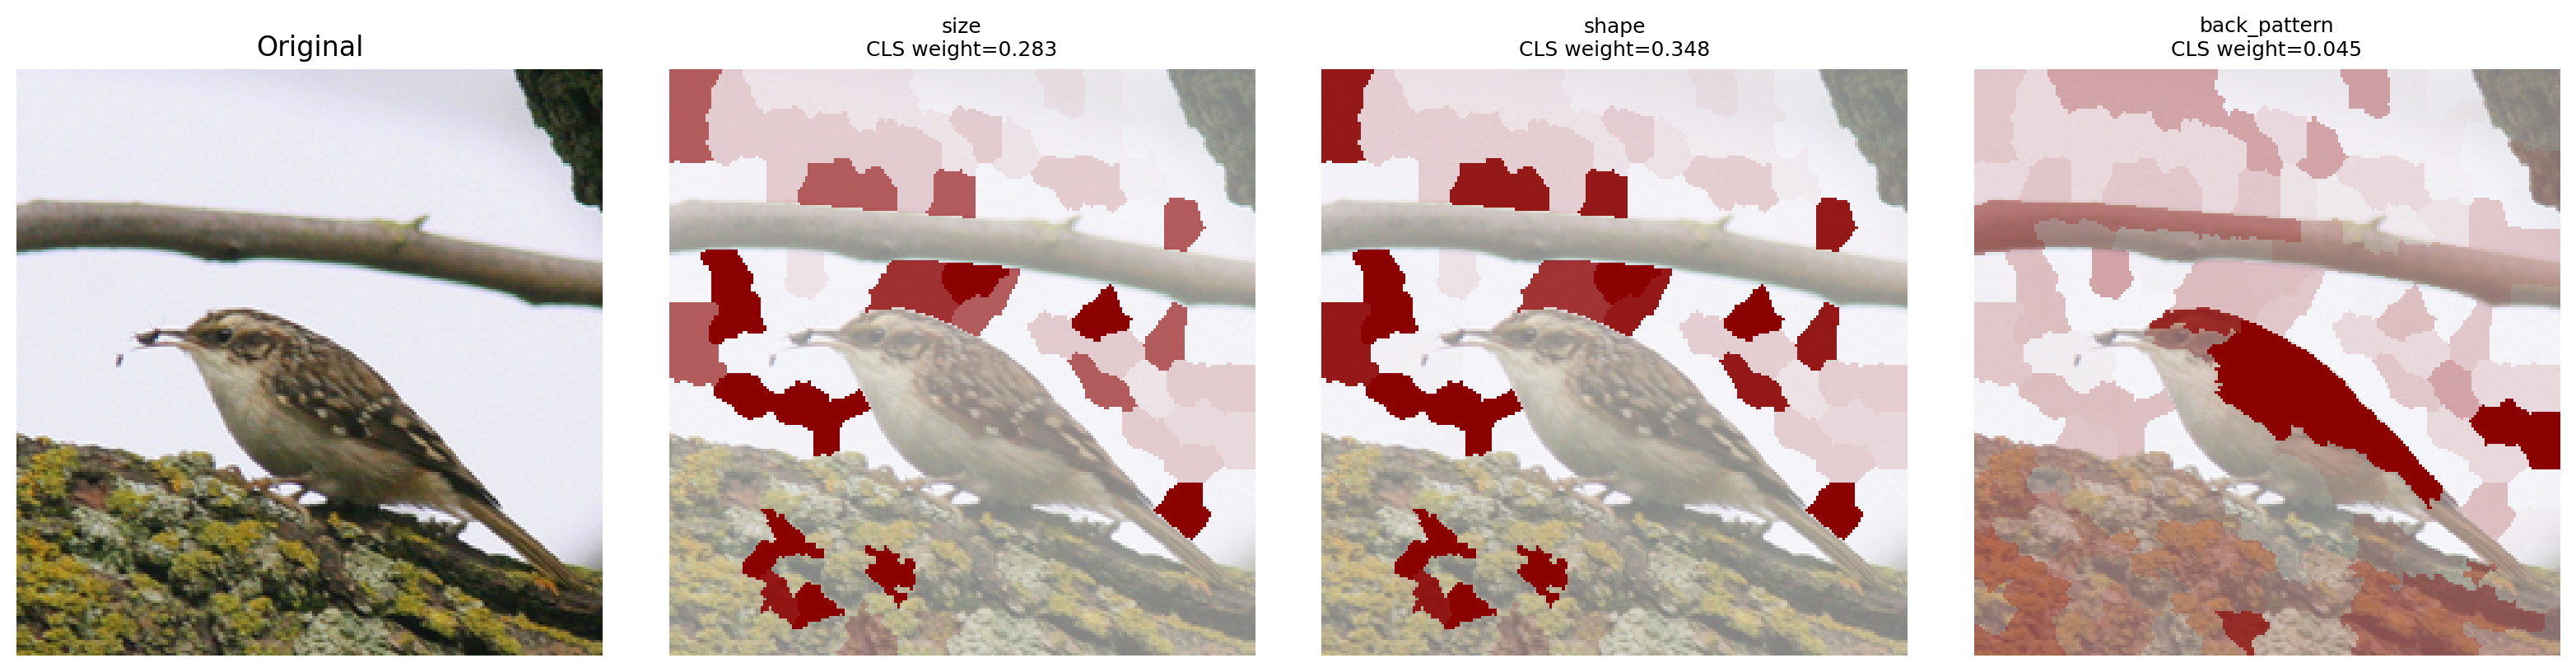
\includegraphics[width=0.92\textwidth]{figures/case_Brown_Creeper_0005_24659_attr_graph_top3_hard.png}
    \caption{Representative limitation case for high-weight global morphology groups. From left to right, the figure shows the original image, the spatial attention map of \textit{shape}, the spatial attention map of \textit{size}, and the spatial attention map of \textit{back pattern}. In this example, the \textit{shape} and \textit{size} queries place substantial attention on background regions. This indicates that these maps should be interpreted as diagnostic internal attention patterns rather than ground-truth localization of size or shape.}
    \label{fig:size_shape_background_example}
\end{figure}

For this reason, the attention visualizations are treated as diagnostic evidence rather than localization evidence. The model is trained with class-level attribute supervision and does not use pixel-level attribute localization labels. Therefore, it is not explicitly forced to align each attribute query with the corresponding semantic bird part. The main conclusion of this thesis is based on the quantitative results, ablation studies, and prediction-level case analysis, while the attention visualization is used only to better understand the internal behavior and limitations of the proposed module.


\subsection{Discussion}

The qualitative and diagnostic analyses provide a more detailed view of the quantitative results. The prediction-level case analysis shows that the proposed model corrects more species-level errors than it introduces. Specifically, it corrects 236 species-level errors made by the H-CAST rerun, while introducing 161 new species-level errors where H-CAST was originally correct. This results in a net gain of 75 correctly classified test images. Over 5,794 test images, this corresponds to approximately 1.29 percentage points, which is consistent with the observed species accuracy improvement from 84.55\% to 85.83\%.

The analysis also shows that many of the corrected cases are intra-family confusions. Among the 236 corrected species-level errors, 194 cases correspond to images where H-CAST predicts the correct family but the wrong species. This accounts for approximately 82.2\% of the corrected cases. This observation is consistent with the motivation of the proposed hard-sibling-aware attribute selection strategy, which is designed to prioritize attributes that help distinguish visually related species within the same family.

However, the proposed method is not uniformly better than the image-only H-CAST baseline. Some predictions that are correct in H-CAST become incorrect in the proposed model, and 659 images remain misclassified by both models at the species level. This indicates that attribute-guided fusion changes the species-level decision boundary and can improve average performance without improving every individual prediction. Therefore, the proposed method should be interpreted as improving species-level recognition overall, especially for some intra-family confusions, rather than as a model that consistently corrects all fine-grained errors.

The path-consistency analysis also helps explain the trade-off observed in the quantitative results. There are 86 images where the proposed model predicts the correct species but the full hierarchical path is still inconsistent. This is consistent with the fact that the proposed model achieves strong species accuracy, FPA, and wAP in the main setting, but does not obtain the lowest TICE among all ablation settings. Since attribute-guided fusion is applied mainly to the species-level branch, it can improve fine-grained species discrimination without necessarily improving taxonomy consistency in every case.

Finally, the attention analysis highlights an important limitation of the current approach. Although the attribute-guided branch improves classification performance, the attention visualizations do not provide strong evidence of precise semantic attribute localization. Global groups such as \textit{size} and \textit{shape} often dominate the pooling attention, and their spatial maps can be diffuse or include background regions. Some local attribute queries attend to plausible bird regions, but this behavior is not sufficiently consistent to support a strong localization claim. This suggests that the model may use a combination of object-part cues, global morphology, silhouette, scale, and contextual information.

Overall, the qualitative analysis supports the main conclusion of this thesis: attribute-guided fusion improves the main quantitative performance of H-CAST, especially species accuracy, FPA, and wAP, and many of the corrected errors are intra-family species confusions. At the same time, the diagnostic attention analysis shows that the current method should not be interpreted as a precise attribute localization model. Future work could address this limitation by incorporating object masks, part annotations, stronger localization constraints, or attention regularization methods that encourage attribute queries to focus more consistently on bird regions.


